\documentclass{ci5652}
\usepackage{graphicx,amssymb,amsmath}
\usepackage[utf8]{inputenc}
\usepackage[spanish]{babel}
\usepackage{hyperref}
\usepackage{subfigure}
\usepackage{paralist}
\usepackage[ruled,vlined,linesnumbered]{algorithm2e}
\usepackage{graphicx}

\setlength{\parskip}{0.5em}

\graphicspath{ {./images/} }

%----------------------- Macros and Definitions --------------------------

% Add all additional macros here, do NOT include any additional files.

% The environments theorem (Theorem), invar (Invariant), lemma (Lemma),
% cor (Corollary), obs (Observation), conj (Conjecture), and prop
% (Proposition) are already defined in the ci5652.cls file.

%----------------------- Title -------------------------------------------

\title{Estudio de Aplicación de Metaheurísticas al \\ problema Maximum Diversity Problem (MDP)}

\author{Cristian Medina
        \and
        Manuel Pacheco}

%------------------------------ Text -------------------------------------

\begin{document}
\thispagestyle{empty}
\maketitle


\begin{abstract}
El problema de máxima diversidad (Maximum Diversity Problem), consiste en elegir M elementos de un conjunto de N elementos tal que las suma de las distancias entre los elementos elegidos sea la máxima posible. Catalogado como un problema NP-Hard en 1993 por Kou, Glover y Dhit, el problema está formalmente estipulado bajo la siguiente fórmulas de función objetivo a maximizar y restricción de tamaño:

$$\sum_{i=1}^{n-1} \sum_{j=i+1}^n d_{ij}x_ix_j$$
$$\sum_{i=1}^{n}x_i<m$$ 
Donde $n$ es la cardinalidad de elementos del conjunto, $m$ la cantidad de elementos elegidos, $d_{ij}$ es la distancia entre el elemento $i$ y el elemento $j$, $x_i$ es una función booleana que toma el valor de 1 si el elemento $i$ fue elegido, 0 si no fue elegido. Estas definiciones son las utilizadas en menciones posteriores en caso de omitirse una definición en el momento.
 
Las aplicaciones de este problema se pueden  encontrar en estudios genéticos, sistemas ecológicos, controles de inmigración, tratamientos médicos, entre otros. Ha sido un caso de estudio para la aplicación de heurísticas y metaheurísticas, particularmente para la búsqueda local. Fue catalogado como un problema NP-Hard en 1993 por Kou, Glover y Dhit al reducir el problema de clique a MDP.

El presente artículo presenta un estudio sencillo de la aplicación de metaheurísticas para la resolución de este problema. Se realiza un estudio comparativo de las técnicas de Local Search (LS), Iterated Local Search (ILS), Tabu Search (TS), Genetic Algorithm (GA) y Scatter Search (SS) en las intancias del problema en los sets SOM, GKD y MDG de MDPLIB de optsicom.es.

\end{abstract}

\section{Trabajos Previos}
El problema de máxima diversidad ha sido estudiado aplicando múltiples heurísticas y metahaurísticas. En general todas las heurísticas estudiadas presentan buenos resultados, sin embargo, se destacan las de búsqueda local al poseer resultados de mejor calidad para la mayor parte de los casos de prueba.

Se destaca en particular el Basic VNS por Brimberg~\cite{vnsbrimberg}. Este consiste en una estructura de datos eficiente que representa los conjuntos de datos actualizados, del cual genera aleatoriamente una solución parcial a la cual le aplica una búsqueda local intercambiando los elementos de su solución con los elementos no incluidos.
En un segundo lugar, se encuentra el VNS implementado por Aringhieri y Cordone~\cite{vnsarincor}, el cual consiste en una construcción de una solución con un método greedy y un posterior procesamiento cambiando k elementos de la solución y aplicando una búsqueda tabú simple sobre esta.

Para casos de prueba de mayor tamaño, se destaca las búsquedas en Tabú. Un ejemplo de esta es la presentada por Palubeckis~\cite{palubeckis}, una búsqueda Tabú iterativa que alterna entre búsqueda tabú y técnicas de perturbación. Cuando la búsqueda Tabú encuentra un resultado mejor al inicial, utiliza una búsqueda local a la nueva solución. Su método de perturbación es una selección de elementos aleatorios del conjunto para viajar por el espacio de soluciones. Para casos pequeños este método se desempeña bien, pero no es el mejor.

Cabe destacar también los estrategias GRASP desarrolladas por Silva et~\cite{silva}, donde se construye una solución parcial inicial y se mejora de forma iterativa; y la propuesta por Duarte y Martí~\cite{duarmar}, que parten de la heurística propuesta por Glover de C2 y D2, aplicándole su propia metodología GRASP.

\section{Representación de la solución}
Para la representación de una solución del problema se utilizan dos alternativas. Para los algoritmos LS, ILS, TS y SS se optó por una representación compacta.
Sea el conjunto de elementos de tamaño $n$ y la solución de tamaño $m$, se opta por representar la solución como un vector de tamaño $m$ donde cada componente contiene la etiqueta del elemento escogido. Para GA se utiliza una representación completa: un vector de tamaño $n$ donde cada componente está permanentemente asociada a un elemento del problema e indica si pertenece o no a la solución (i.e. un $x_i$ como en la descripción del problema).

\section{Solución Inicial}
Dependiendo de la metaheurística a utilizar se usan métodos de construcción de las soluciones iniciales de forma diferente. La primera es la clásica solución aleatoria: se seleccionan los elementos que pertenecen a la solución al azar. La segunda sigue un principio de intuición que denominamos $Potencial$ de un elemento definida de la siguiente forma:

$$P(i)=\sum_{j=1}^{n}d_{ij}$$

De manera informal, el $Potencial$ de un elemento indica cuánto aporta a la función objetivo si se tomasen en cuenta todas las conexiones con todos los demás elementos. Por tanto, elegimos los primeros $m$ nodos que tengan mayor potencial. Definimos a esta estrategia como solución inicial greedy.

En la mayoría de los problemas trabajados, las soluciones aleatorias rondan generalmente entre 50\% y 75\% del valor de las mejores soluciones encontradas en la librería (soluciones referencia), dependiendo del tamaño del problema, siendo las peores las de problemas más grandes. La solución greedy supera el 95\% y tiende a llegar tan alto como 98\% de la solución referencia.

En la mayoría de los problemas se intenta utilizar la solución greedy sobre la aleatoria. Para LS, ILS y TS se utiliza greedy. Para las metaheurísticas poblacionales GA y SS, se inicia con soluciones aleatorias.

\section{Local Search}
El primer algoritmo implementado consiste en Búsqueda Local. Durante la búsqueda, el objetivo es mejorar una solución existente modificando aquellos elementos que lleven la solución a acercarse a un óptimo (al menos de forma local).

La implementación de LS esta basada en el uso de $k\text{--}opt$, con 4 características en las cuales hacer énfasis:
\begin{itemize} \itemsep5pt
	\item Se busca mejorar los $m$ componentes de la solución.
	\item Los vecinos de cada componente son definidos en base al tamaño $n$ del problema.
	\item Cada componente es reemplazada por el mejor candidato encontrado
	\item La búsqueda por componente se detiene si ha pasado un numero de iteraciones sin conseguir una solución candidata que mejore la solución actual.
\end{itemize}

\subsection{Algoritmo de Local Search}
El algoritmo utilizado es equivalente al aquí mostrado, abstrayendo las particularidades de implementación y optimización del algoritmo. Esto aplica a todos los algoritmos mostrados en el presente documento.

\begin{algorithm}
\DontPrintSemicolon
$S \leftarrow$ Solucion existente\;
$S_i \leftarrow$ elemento $i$ de la solucion\;
$U \leftarrow$ elementos no escogidos\;
$P \leftarrow$ elementos del problema\;
\Begin{
	\ForEach{$i \in |S|$ de derecha a izquierda}{
		$U' \leftarrow$ NH\_SIZE elementos aleatorios de U\;
		\ForEach{$u \in U'$}{
			$S' \leftarrow$ S con $S_i$ reemplazado por u\;
			\If{$valor(S') > valor(S)$}{
				$S \leftarrow S'$\;
				Marcar $u$ como mejor candidato
			}
			\If{pasan MAX\_REPEATS iteraciones sin marcar $u$}{
				break\;
			}
		}			
	}	
}
\end{algorithm}

Para $NH\_SIZE$ y $MAX\_REPEATS$ se entonaron los valores de $\frac{|P|-|S|}{5}$ y $30$ respectivamente.

\begin{algorithm}
  \DontPrintSemicolon
  \vspace*{0.1cm}
  $V \leftarrow$ vector de arcos\;
  $S \leftarrow$ vector solución inicial\;
  $C \leftarrow$ vector de elementos no elegidos\;
  $IS \leftarrow \emptyset$ // conjunto de cambios probados\;
  $Itera \leftarrow true$ // cota de salida\;
  $localIter \leftarrow 0$\;
  $totalIter \leftarrow 0$\;
  $pivote \leftarrow |S|-1$\;
  $distanciaActual = Distancia(S)$\;
  \While{true}{
    \eIf{$localIter < MAX\_LOCAL\_LITER \land localIter < |Nodos| - |S|$}{
      $NodoAleatorio \leftarrow Rand(C)$\;
      \If{$NodoAleatorio \in IS$}{
        \textbf{continue}\;
      }
      IS $\leftarrow IS \cup \{NodoAleatorio\}$\;
      $respaldo \leftarrow pivote$\;
      $pivote \leftarrow nodoAleatorio$\;
      \eIf{$Distancia(S) > distanciaActual$}{
        $DistanciaActual = Distancia(S)$\;
        $C = C - nodoAleatorio + respaldo$\;
      }{
        $pivote = Respaldo$\;
      }
      $localIter++$\;
      $totalIter++$\;
    }{
      $IS \leftarrow \emptyset$\;
      $localIter = 0$\;
      $pivote--$\;
    }
    \If{$totalIter > MAX\_ITER \lor pivote < 0$}{
      \KwRet{$distanciaActual$}\;
    }
  }
\end{algorithm}



















\begin{figure}[p]
	\setlength\fboxsep{0pt}
	\setlength\fboxrule{0.5pt}
	\fbox{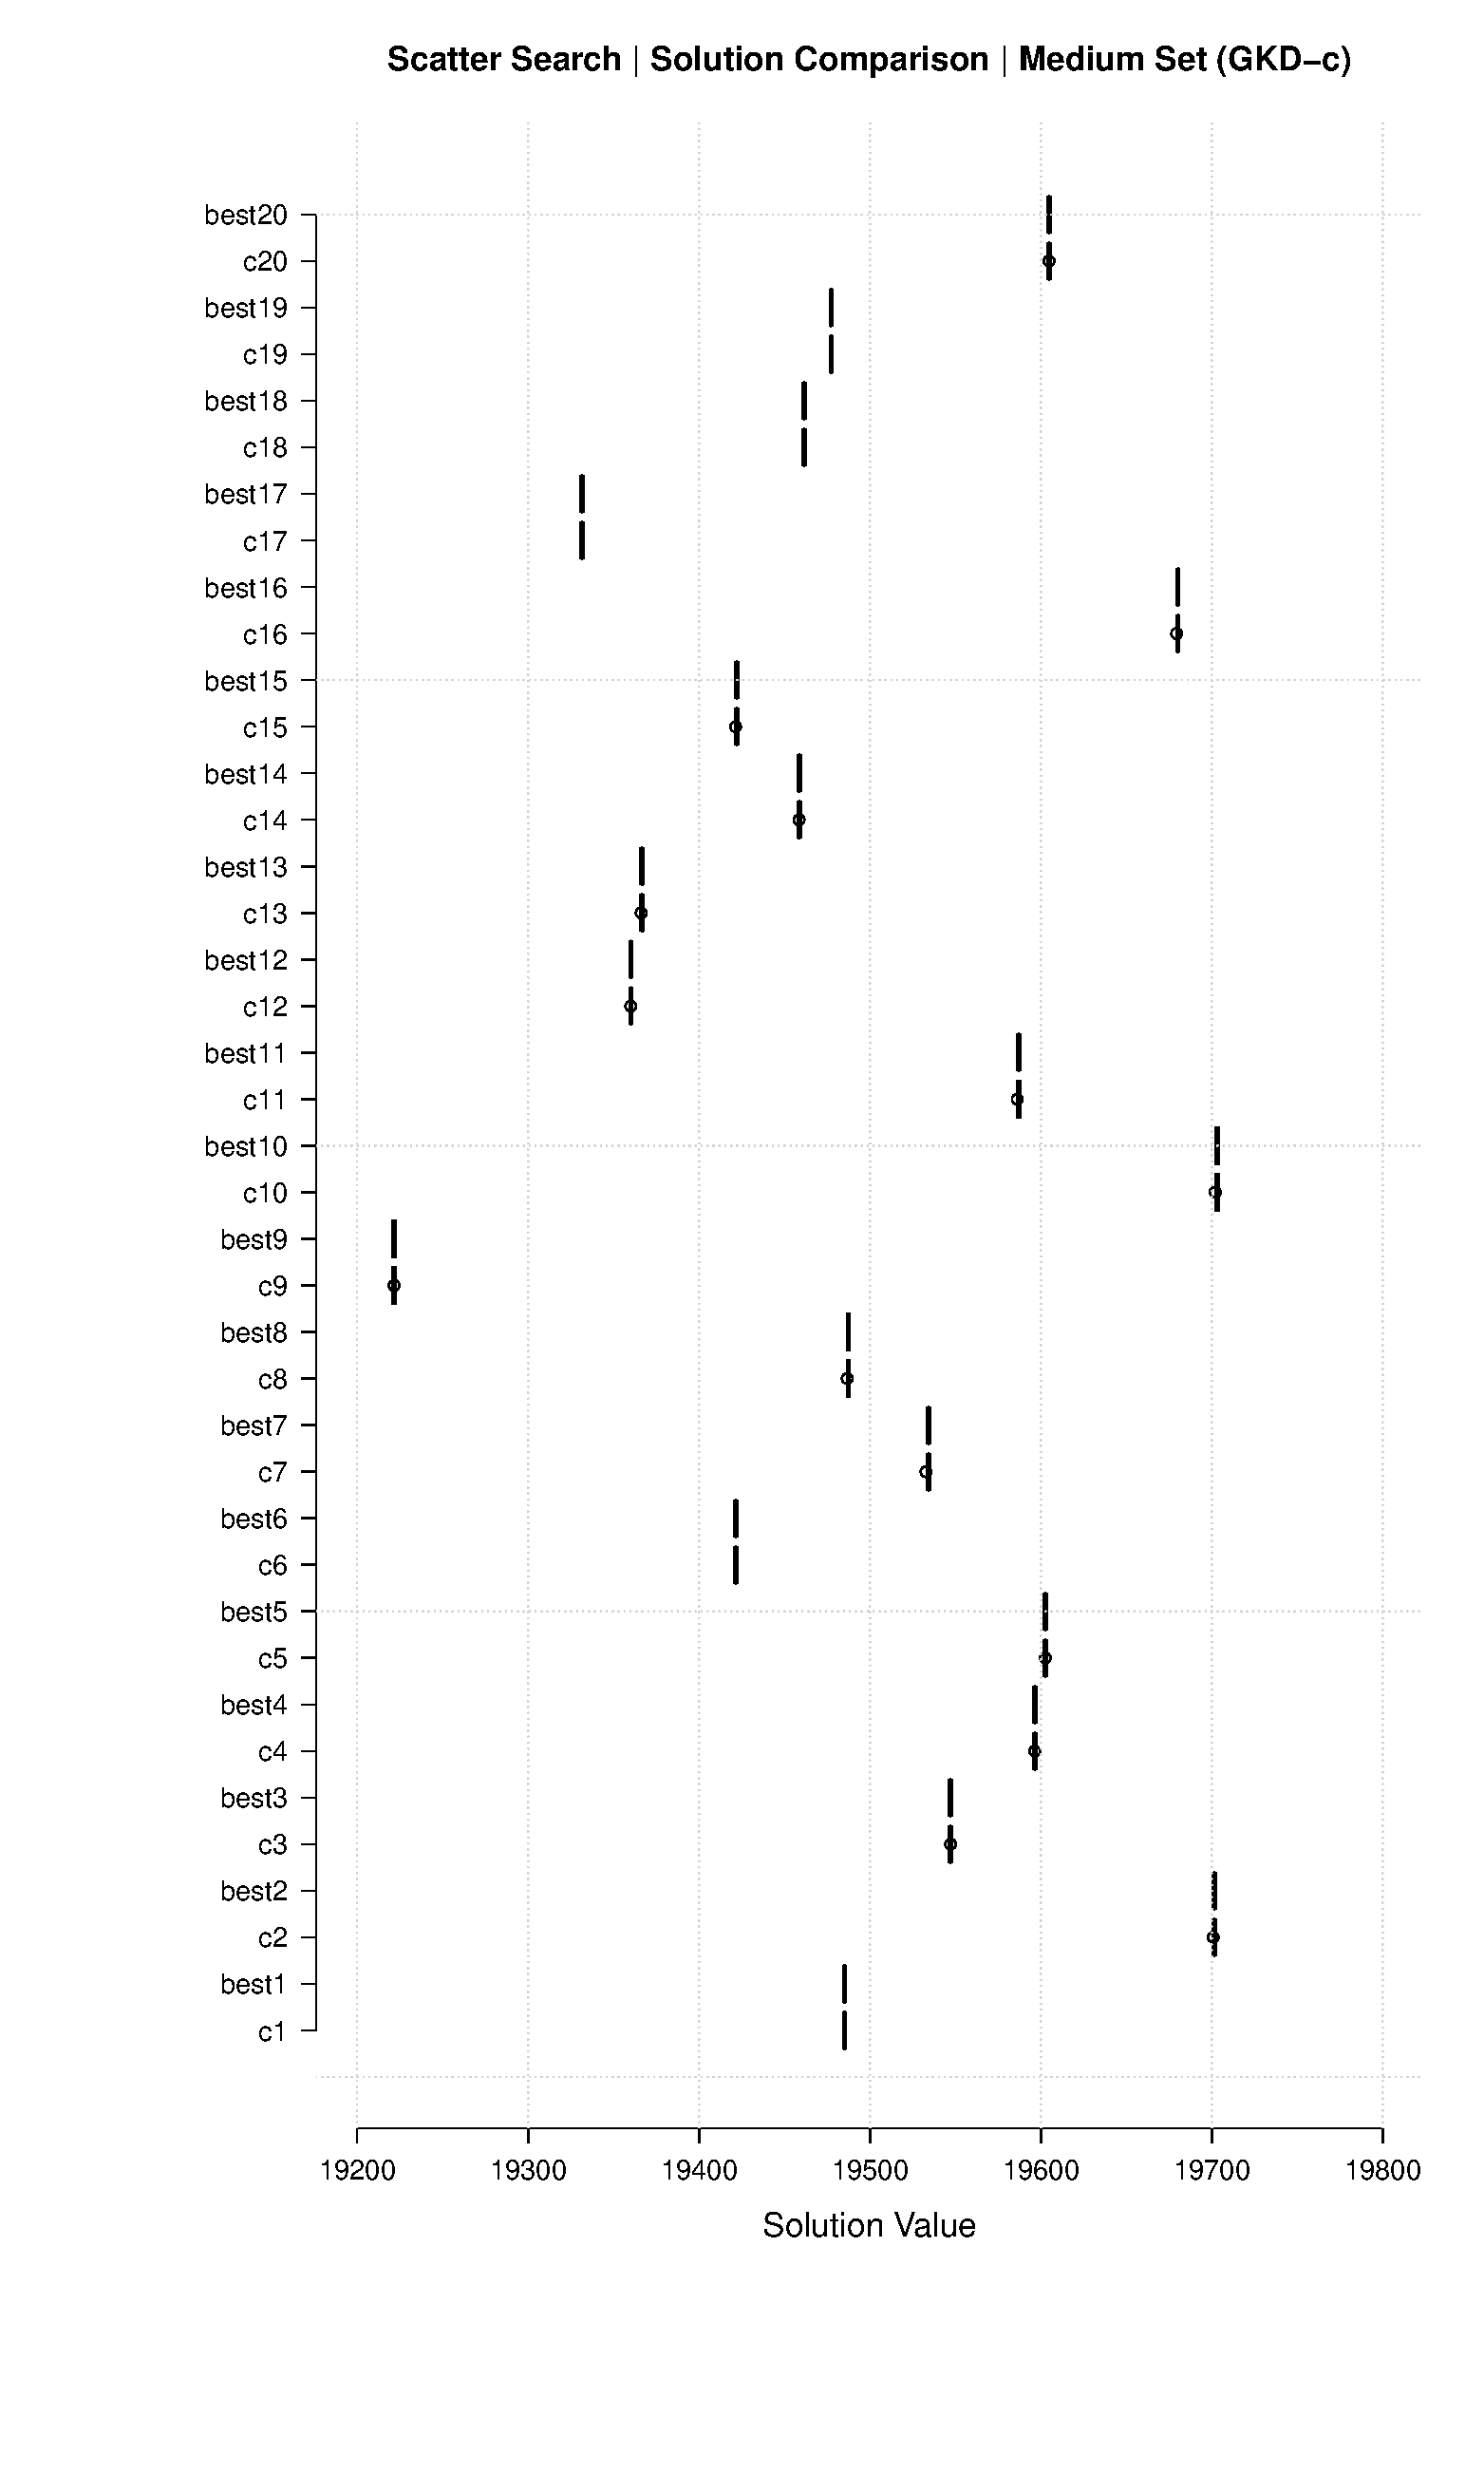
\includegraphics[width=\linewidth]{scatter-solution-medium}}
	\caption{Comparación de soluciones de SS en problemas de tamaño mediano.}
	\label{fig:ss_s_m}
	\label{fig:ss_s_m}
\end{figure}

\section{Búsqueda ILS}
En la implementación de la metaheurística de búsqueda local iterativa, a partir de una solución inicial, comienza un ciclo de donde se perturba la mejor solución, se mejora esa solución parcial y se comparan las soluciones. La perturbación consiste en intercambiar aleatoriamente \textit{k} nodos de la solución parcial por nodos no elegidos. El mejoramiento es realizar una búsqueda local a la solución obtenida por la perturbación. Luego se compara la solución parcial con la mejor solución obtenida, y se actualiza la segundar de ser mejor la solución parcial.

Si transcurren \textit{h} ciclos sin que mejore la solución, se procede a aumentar la perturbación, aumentando en uno el \textit{k}. Este ciclo ocurre hasta que se cumpla un número máximo de iteraciones, o el valor \textit{k} de las perturbaciones supera el tamaño de la solución.

%\section{Algoritmo de Búsqueda Local Iterativa}
%\begin{algorithm}
%  \DontPrintSemicolon
%  \vspace*{0.1cm}
%	$C \leftarrow$ conjunto nodos no escogidos\;
%  $S \leftarrow$ conjunto de nodos de la solución inicial\;	//Solucion Parcial
%	$BS \leftarrow$ S\;	//Mejor solucion
%  $k \leftarrow$ PERTURBACION_INCIAL\;
%	$m \leftarrow$ TAMAÑO_DE_SOLUCION\;
%	$numIteraciones \leftarrow$ 0\;
%	$intentosK \leftarrow$ 0\;
%  \While{numIteraciones < MAX_ITERACIONES \land k < m}{
%
%		$elemEscogido \leftarrwo$ \emptyset$\;
%		\for {i=0 hasta k}{
%			$elemEntrando \leftarrow$ x aleatorio tal que, x \subset C, x \not\subset elemEscogido, x \not\subset S,\;
%			$elemSalida \leftarrow$ x aleatorio tal que, x \not\subset C, x \not\subset elemEscogido, x \subset S,\;
%			$elemEscogido \leftarrwo$ \cup elemEntrada \cup elemSalida\;
%			$S \leftarrow (S - elemSalida) \cup elemEntrada\;
%			$C \leftarrow (S - elemEntrada) \cup elemSalida\;
%		}
%		$S \leftarrow busquedaLocal(S)\;
%		\If{$distancia(S) > distancia(BS)$}{
%        $BS \leftarrow$ S\;
%				$intentosK \leftarrow$ 0\;
%      }
%    \eIf{}{
%			\If{$intentosK > MAX_INTENTOS_K}{
%				$k \leftarrow$ k + 1\;
%				$intentosK \leftarrow$ 0\;
%      }
%    	\eIf{}{
%				$intentosK \leftarrow$ intentosK + 1\;
%	    }
%			$S \leftarrow$ BS\;
%    }
%		$numIteraciones \leftarrow$ numIteraciones+1\;
%	}
%
%\end{algorithm}

\section{Resultados}
Para el estudio del desempeño de los algoriymos, se ejecuto 15 veces cada caso de preuba y se promediaron
los datos obtenidos. Se consideran los casos de prueba GDK-c que consiten en puntos generados aleatorios y
sus respectivas distancias euclidianas entre si, con una cantidad de nodos igual a 500 y una solución de tamaño 50.
También se consideran 5 casos de SOM-b, con una cantidad de nodos entre 100 y 200, soluciones de tamaño 10 a 40, que consisten
en arcos generados aleatoriamente, extraídos de una distribucion uniforme. Igualmente se usan los casos de MDG-a, que
son arcos enteros entre 0 y 10 sacados aleatoriamente de una distribución uniforme, con problemas con 500 nodos y 50 de tamaño de soluciones, y sus 3 de sus versiones más grandes de 2000 nodos y 200 de tamaño de solución

En general los resultados dados con ILS superan en calidad a los presentado solo con Búsquedad Local.
Esto ocurre tanto con soluciones iniciales aleatorias como con soluciones iniciales con el procesamiento
greedy antes descrito. Sin embargo su costo de tiempo es considerablemente mayor. En particular con los casos
más grandes, MDG-a de 2000 nodos,ILS llega a tardar 10 minutos a diferencia d LS que tarda poco más de un segundo,
con una diferencia de 2% de error relativo favorable a ILS. También se observa que los resultados dados
por las corridas con la solución inicial greedy obtienen mejores resultados que con soluciones iniciales
aleatorias.



%---------------------------- Bibliography -------------------------------

% Please add the contents of the .bbl file that you generate,  or add bibitem entries manually if you like.
% The entries should be in alphabetical order
\small
\bibliographystyle{abbrv}

\begin{thebibliography}{99}

\bibitem{vnsbrimberg}
Brimberg, J., N. Mladenovic, D. Urosevic and E. Ngai. (2009).
\newblock Variable neighborhood search for the heaviest k-subgraph.
\newblock {\em Computers $\&$ Operations Research}, 36(11): 2885-2891.

\bibitem{vnsarincor}
R. Aringhieri and R. Cordone.
\newblock Better and faster solutions for the maximum diversity problem.
\newblock {\em Technical report, Universit degli Studi di Milano, Polo Didattico e di Ricerca di Crema}, 2006.

\bibitem{silva}
G.C. Silva, M.R.Q. Andrade, L.S. Ochi, S.L. Martins, and A. Plastino.
\newblock New heuristics for the maximum diversity problem.
\newblock {\em Journal of Heuristics}, 13(4):315–336, 2007.

\bibitem{duarmar}
R. Aringhieri, R. Cordone, and Y. Melzani.
\newblock Tabu search vs. grasp for the maximum diversity problem.
\newblock {\em A Quarterly Journal of Operations Research}, 6(1):45–60, 2008.

\bibitem{palubeckis}
G. Palubeckis.
\newblock Iterated tabu search for the maximum diversity problem.
\newblock {\em Applied Mathematics and Computation}, 189:371383, 2007.




\end{thebibliography}

\end{document}
